\setchapterpreamble[u]{\margintoc}
\chapter*{Introducción}
\labch{introduction_spanish}
\label{sec:introduction_spanish}

\lettrine[findent=0pt, lines=3]{\fbox{\textbf{L}}}{ }a teledetección ayuda a controlar, predecir y optimizar las actividades de las que dependen procesos del mundo real, y por tanto, a actuar en función de los datos analizados. Existen numerosos sensores que posibilitan esta tarea, los cuales pueden clasificarse en función de la distancia a la que operan, el intervalo de longitudes de onda al que es sensible y el mecanismo de adquisición de datos, ya sea pasivo o activo. Las dos últimas clasificaciones se fundamentan en el mecanismo implementado en el dispositivo. Sin embargo, la primera categoría dependerá de los objetivos y el área de aplicación que persigan tanto los investigadores como el consumidor final. Igualmente, también influyen el presupuesto del que se dispone, y el tamaño y las condiciones ambientales de la zona de estudio, entre otros factores. A pesar de que es posible utilizar sensores que precisan de contacto directo con la superficie objetivo, para medir variables como humedad, temperatura o cantidad de lluvia, este tipo de dispositivos requieren un alto grado de mantenimiento y son más propensos a deteriorarse en condiciones ambientales adversas \cite{silva_low-cost_2019, morais_versatile_2021}. Además, cada uno de estos sensores comunica información de una posición muy específica dentro y fuera de una red de sensores, en lugar de intercambiar datos que conciernen a áreas de grandes dimensiones. Es evidente que en un espacio continuo e infinito, se debe discretizar la monitorización mediante un número variable de posiciones. La disposición de estos sensores, tanto lógica como física, debe ser cuidadosamente diseñada para permitir la intra y extra-comunicación, involucrando nodos a diferentes niveles de la topología propuesta. Por lo tanto, este tipo de tecnologías no son tan apropiadas para aplicaciones de monitorización constante y en tiempo real destinadas a grandes áreas. 

\marginnote[.1cm]{Las técnicas de \textbf{teledetección} evitan las limitaciones espaciales que encontramos en otros dispositivos que aportan medidas mediante contacto directo con la superficie objetivo, o la atmósfera. } 
La teledetección ayuda a mitigar algunas de las desventajas mencionadas, adquiriendo datos desde plataformas aéreas, satelitales e incluso terrestres. Además, no requieren de un contacto directo, sino que simplemente observan y capturan información. La teledetección se define como el arte y la ciencia de adquirir información de objetos y fenómenos sin estar en contacto directo con éstos \cite{lillesand_remote_2015}. De manera similar al ojo humano, los datos se adquieren mediante impulsos generados por estímulos de la luz, los cuales corresponden a unas longitudes de onda específicas. Al menos dos componentes se ven involucrados en el proceso de lectura: sensores y plataformas en las que éstos se acoplan. Los primeros serán objetivo de discusión a lo largo de todo este trabajo, mientras que las plataformas son muy variadas, aunque en un comienzo se limitaban principalmente a satélites. El término \textbf{teledetección} se origina en la década de 1960, acuñado por Eveleyn Pruitt, para referirse a instrumentos satelitales y aéreos que posibilitan medir la radiancia reflejada y emitida. No obstante, las técnicas topográficas fueron ideadas inicialmente en 1849, y llevadas a la práctica en 1858 por F. Tournachon en un globo aerostático, sobrevolando Francia. A partir de aquí, el tamaño de las cámaras se ha ido reduciendo para hacerlas más cómodas de manejar. Otros medios aéreos empleados para estas tareas, influenciados por ciertos acontecimientos históricos y el conocimiento hasta ese momento recabado, fueron cometas (1906; Figura \ref{fig:san_francisco_kite_spanish}), aves (1909), y por último, aeronaves (1908). 

\begin{figure}[!ht]
	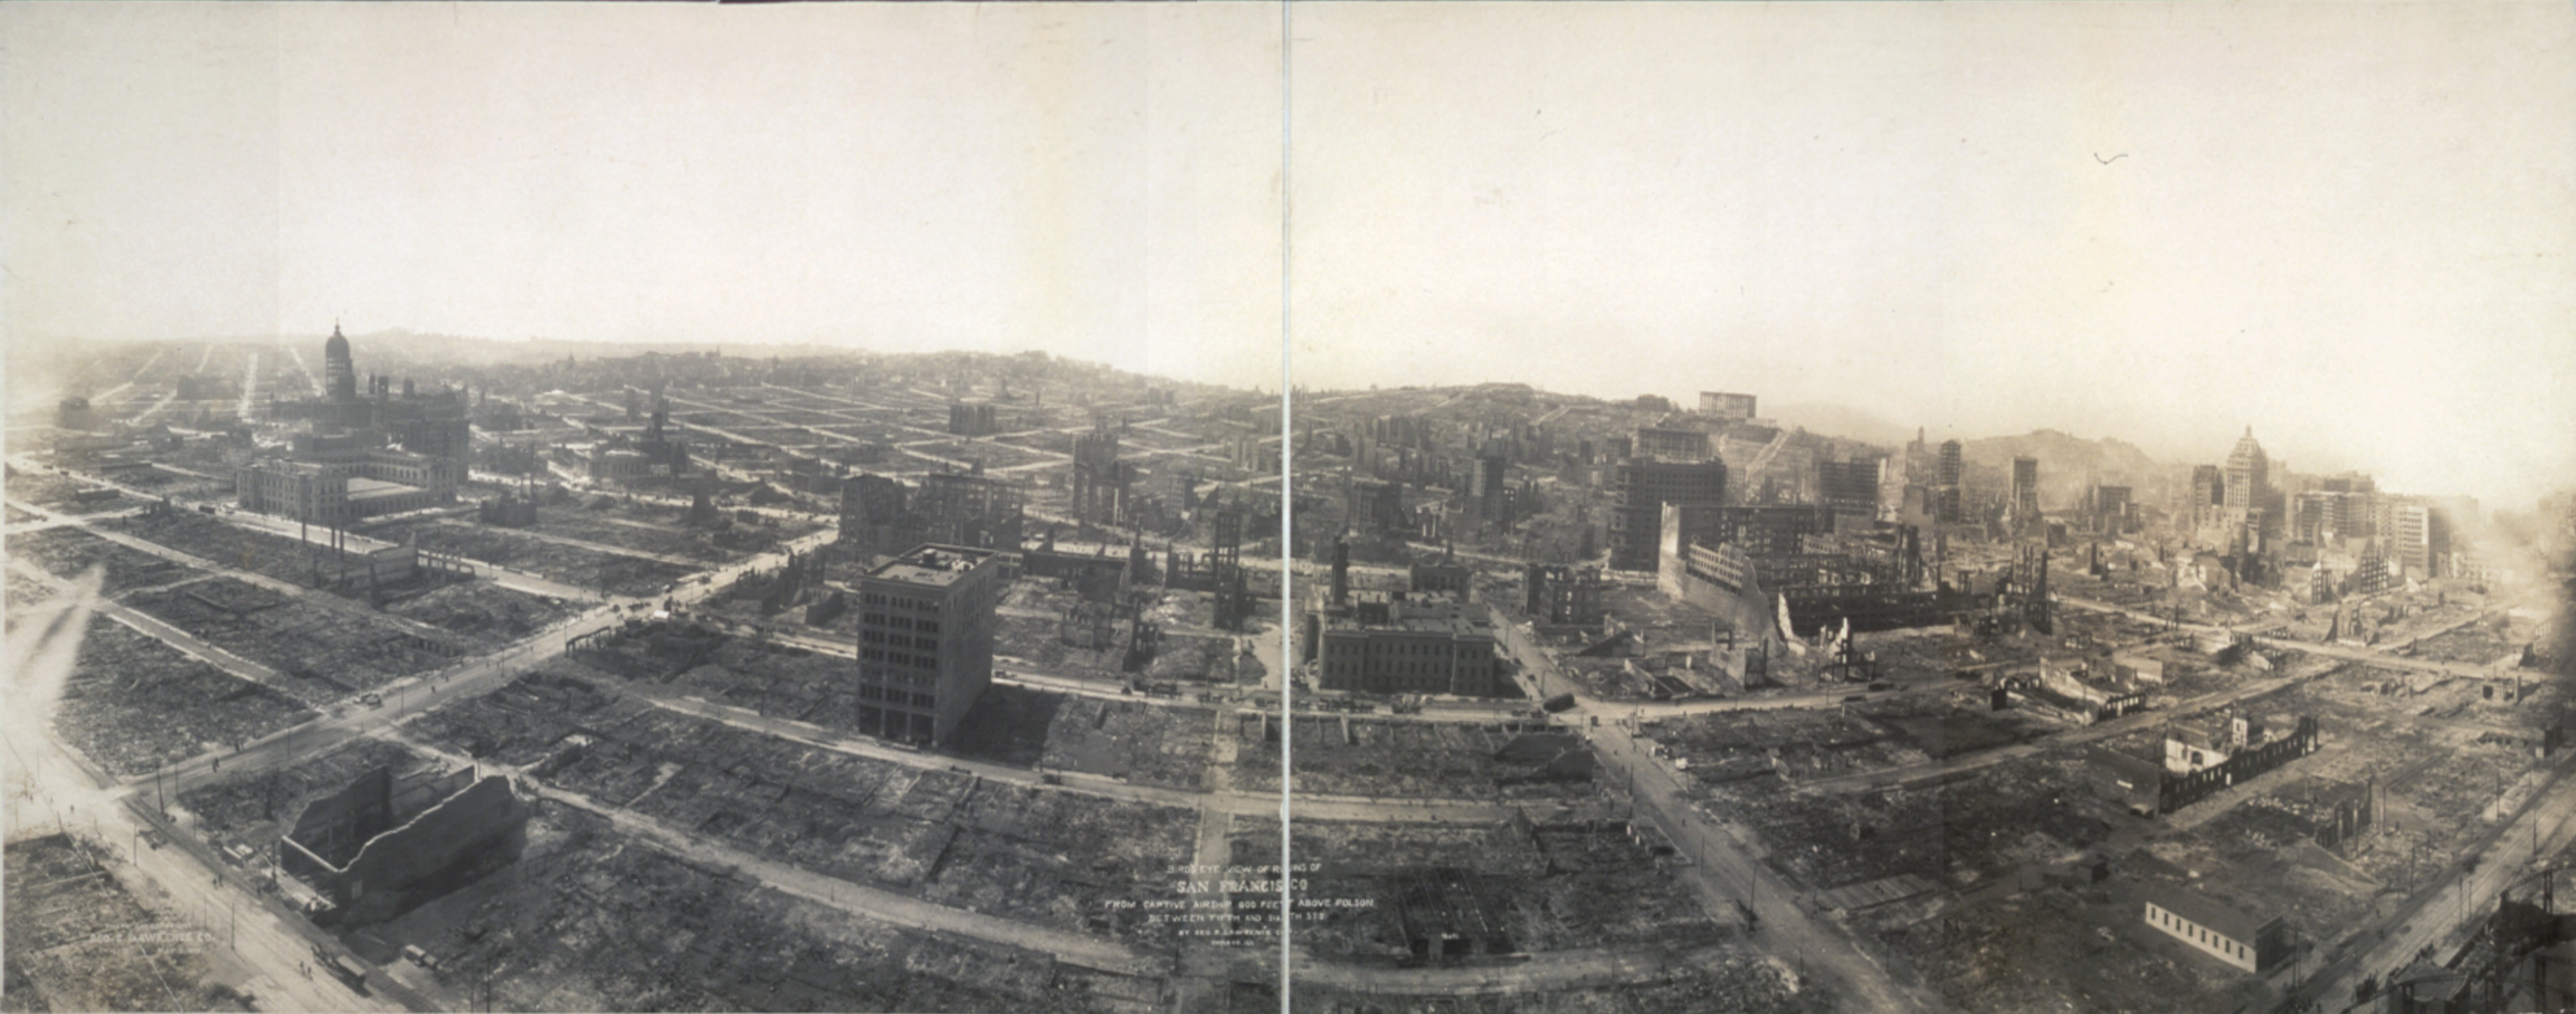
\includegraphics[width=0.95\linewidth]{figs/introduction/san_francisco_kitecamera.jpg}
	\caption{Fotografía de San Francisco después del terremoto de 1906, capturada desde una cámara soportada por siete cometas. }
    \label{fig:san_francisco_kite_spanish}
\end{figure}

La teledetección mediante satélite, tal y como se conoce hoy en día, es posible gracias a la idea inicial de Konstantin Tsiolkovsky de utilizar cohetes para explorar el espacio, publicada bajo el título \textit{Exploring Space using jet propulsion devices}. Esta idea desembocó en el primer lanzamiento con éxito, el satélite Sputnik en 1957, e igualmente contribuyó al desarrollo de satélites para la vigilancia atmosférica. El satélite de observación por televisión e infrarrojos (Television and Infrared Observation Satellite: \acrshort{tiros}) entró en funcionamiento en 1960, integrando un pequeño sistema de infrarrojos y una cámara con un ángulo de visión muy reducido para captar datos en longitudes de onda visibles. En 1978, \acrshort{tiros}-N (n haciendo referencia a "new") supuso un cambio radical tanto en los propios satélites como en los sensores acoplados. Esta misión integraba un radiómetro de alta resolución (1 \si{\kilo\meter}) y podía capturar información en el espectro visible, infrarrojo cercano, infrarrojo medio e infrarrojo térmico. En la actualidad, una versión más avanzada de este satélite opera con el nombre de \acrshort{avhrr} (Advanced Very High-Resolution Radiometer), con una resolución similar y capacidad para capturar seis bandas espectrales diferentes, en lugar de sólo cuatro \cite{national_oceanic_and_atmospheric_administration_avhrr3_nodate}.   

\marginnote[.1cm]{Un amplio repositorio de misiones satelitales se encuentra disponible en el Earth Observation Portal, mantenido por la Agencia Espacial Europea \cite{earth_observation_portal_earth_nodate}.} 
\begin{marginfigure}[3.0cm]
	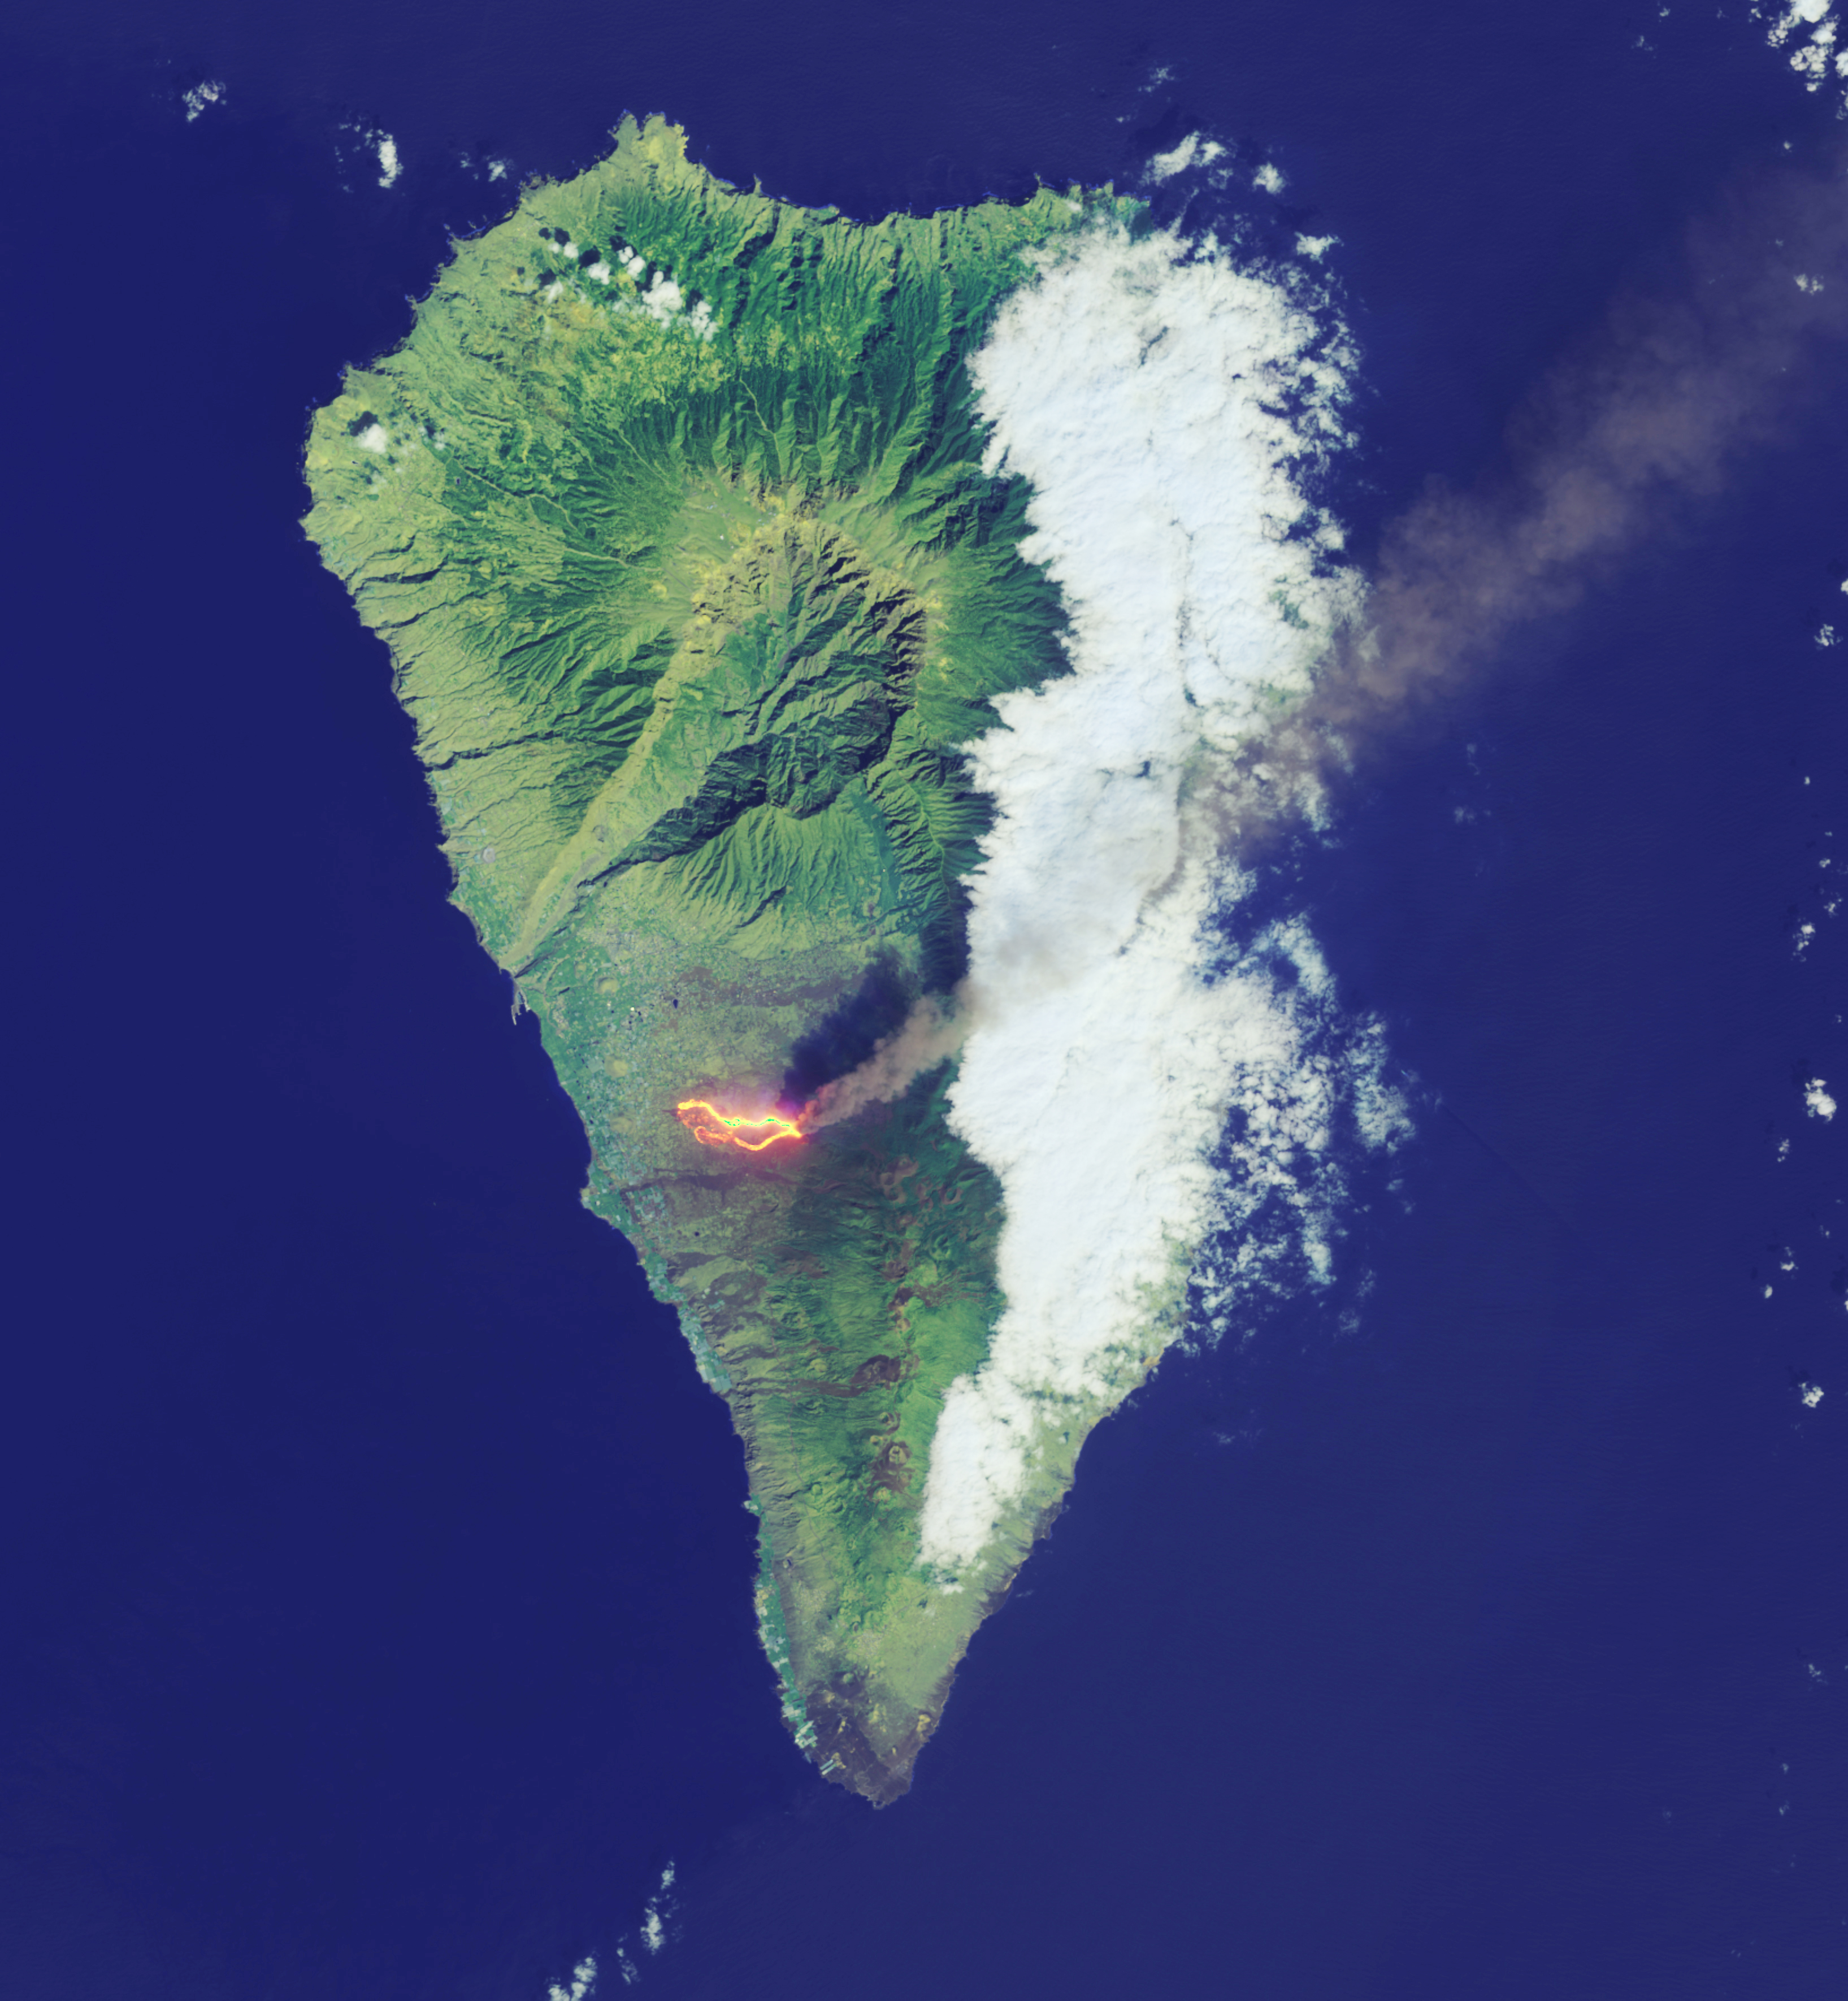
\includegraphics{figs/introduction/landsat8_lapalma.jpg}
	\caption{Erupción del volcán Cumbre Vieja observada desde la misión Landsat-8 \cite{nasa_earth_observatory_lava_2021}.}
	\label{fig:la_palma_landsat8_spanish}
\end{marginfigure}
Entre los proyectos de satélite actualmente operativos, Landsat es el que proporciona la mayor colección de datos de teledetección adquiridos de forma continua. Se utilizó por primera vez como parte del programa NIMBUS de la NASA y en la actualidad hay dos satélites activos, Landsat 8 y Landsat 9, mientras que los otros siete han sido dados de baja o está previsto su desmantelamiento en los próximos años (Landsat 7). La carga útil de Landsat 9 consta de dos sensores: Operational Land Imager (\acrshort{oli2}) y un sensor infrarrojo térmico (\acrshort{tirs2}). Cada día recoge un total de 740 escenas con 11 intervalos espectrales, incluyendo rojo, azul, verde, infrarrojo cercano, infrarrojo de onda corta, térmico, pancromático, costero y de cirros, con una resolución entre 15 \si{\meter} a 100 \si{\meter}. Otros misiones de satélite destacadas son el Satélite de Recursos Terrestres China-Brasil (China–Brazil Earth Resources Satellite: \acrshort{cbers}) y el programa Copernicus, financiado por la Comisión Europea. El satélite CBERS-04A está equipado con tres sensores que capturan cinco intervalos diferentes con una resolución espacial entre 2 \si{\meter} y 55 \si{\meter} \cite{instituto_nacional_de_pesquisas_espaciais_inpecbers_2019}. Por su parte, la misión Sentinel-2 acquire 13 bandas distribuidas en el espectro visible, infrarrojo cercano y de onda corta (ver Figura \ref{fig:sentinel2_spanish}), con una resolución espacial que oscila entre los 10 \si{\meter} y los 60 \si{\meter} \cite{european_environment_agency_eu_2017}. El periodo de tiempo para revisitar el mismo punto de la Tierra es de diez días, en comparación con los 16 días que necesita Landsat 9 o los 31 días de CBERS-04A.

\begin{figure}[!ht]
	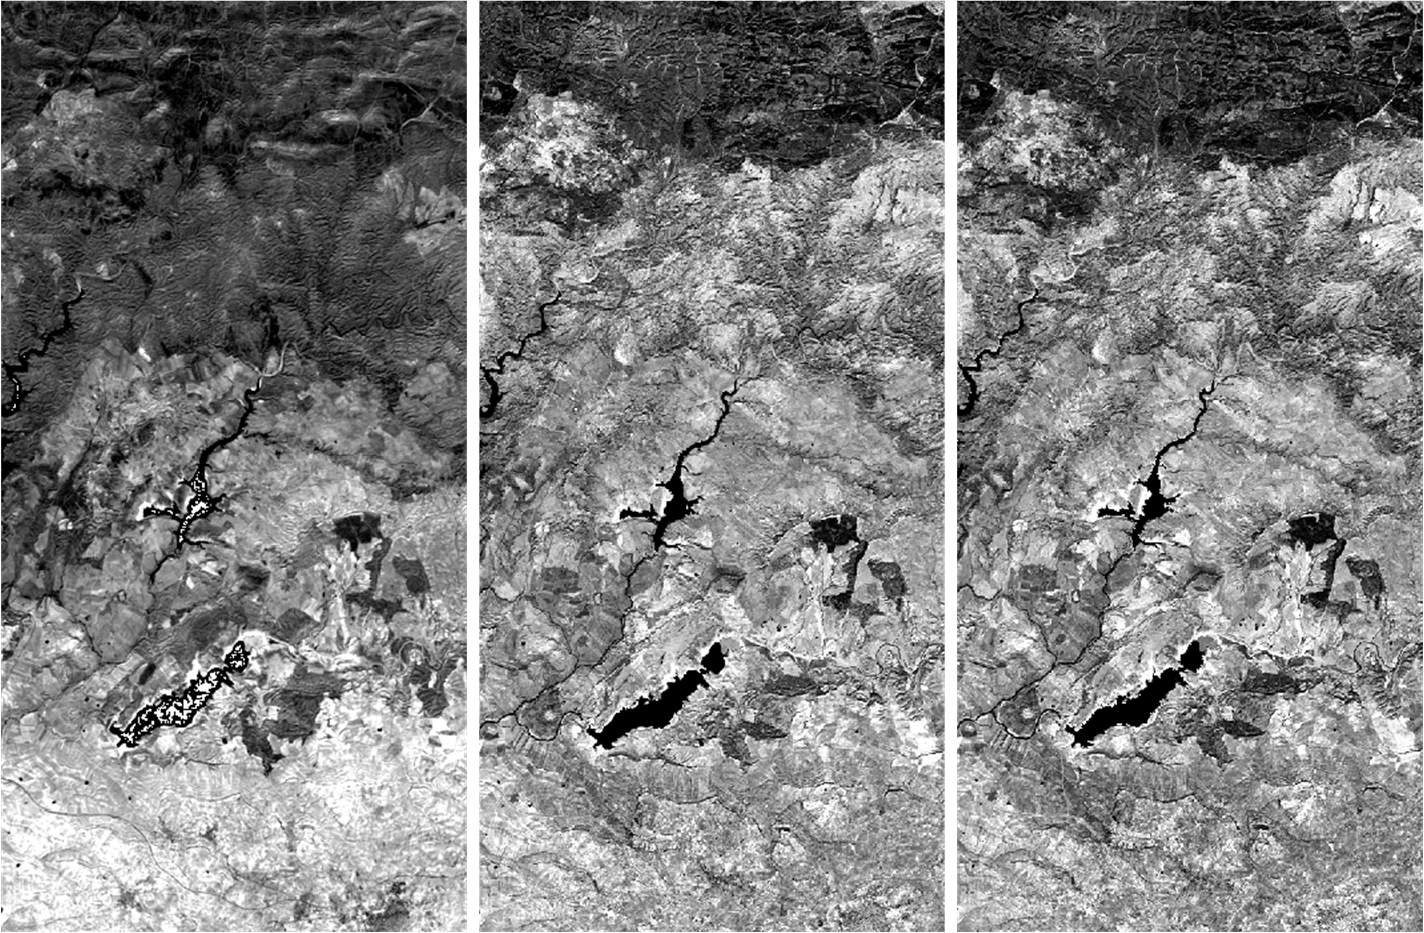
\includegraphics{figs/introduction/sentinel2_bands.png}
	\caption{Tres bandas en el infrarrojo cercano capturadas por la misión Sentinel-2 (banda 9, 935-955 \si{\micro\meter}, banda 11, 1567-1658 \si{\micro\meter}, y banda 12, 2114-2889 \si{\micro\meter}). }
    \label{fig:sentinel2_spanish}
\end{figure}

Por tanto, las imágenes por satélite son más adecuadas para monitorizar cambios a larga escala, utilizando series temporales que abarcan meses, años e incluso décadas. Estos datos permiten comprender la interacción entre el hombre y la naturaleza, así como el impacto de los fenómenos naturales (Figura \ref{fig:la_palma_landsat8_spanish}). Algunas aplicaciones de los conjuntos de datos obtenidos por misiones de satélite son el control del uso del suelo, deforestación, cambios en la superficie terrestre y asentamientos urbanos \cite{asokan_change_2019}. No obstante, la resolución espacial y el periodo para revisitar un mismo punto en satélites no comerciales dificultan su aplicabilidad a tareas de monitorización que requieren de un nivel de detalle elevado (Level of detail: \acrshort{lod}). Este nivel de detalle abarca tanto la resolución espacial como la resolución temporal, o a ambas, siendo éstas las principales limitaciones de las imágenes de satélite, además del elevado coste. A pesar de estas desventajas, el uso de imágenes por satélite está en aumento debido a la disminución paulatina de la distancia representada en un píxel (Ground Sampling Distance: \acrshort{gsd}) y el periodo empleado para revisitar un mismo punto (véase la figura \ref{fig:scopus_search_platforms_spanish}). Por ejemplo, el satélite comercial Pléiades Neo (VHR-2020) de Airbus Defense \& Space \cite{airbus_pleiades_2021} es capaz de adquirir diariamente siete bandas con una resolución de 30 \si{\centi\meter} por píxel. Incluso para las misiones gubernamentales, el ciclo de repetición se puede ver reducido mediante misiones complementarias que operan con órbitas y sensores similares. De esta manera, las misiones Landsat-8 y Landsat-9 obtienen datos de un mismo punto cada 8 días \cite{masek_landsat_2020}. Aun así, obtener datos de misiones espaciales es mucho más prohibitivo en términos económicos que otras técnicas.

\begin{figure}[!ht]
	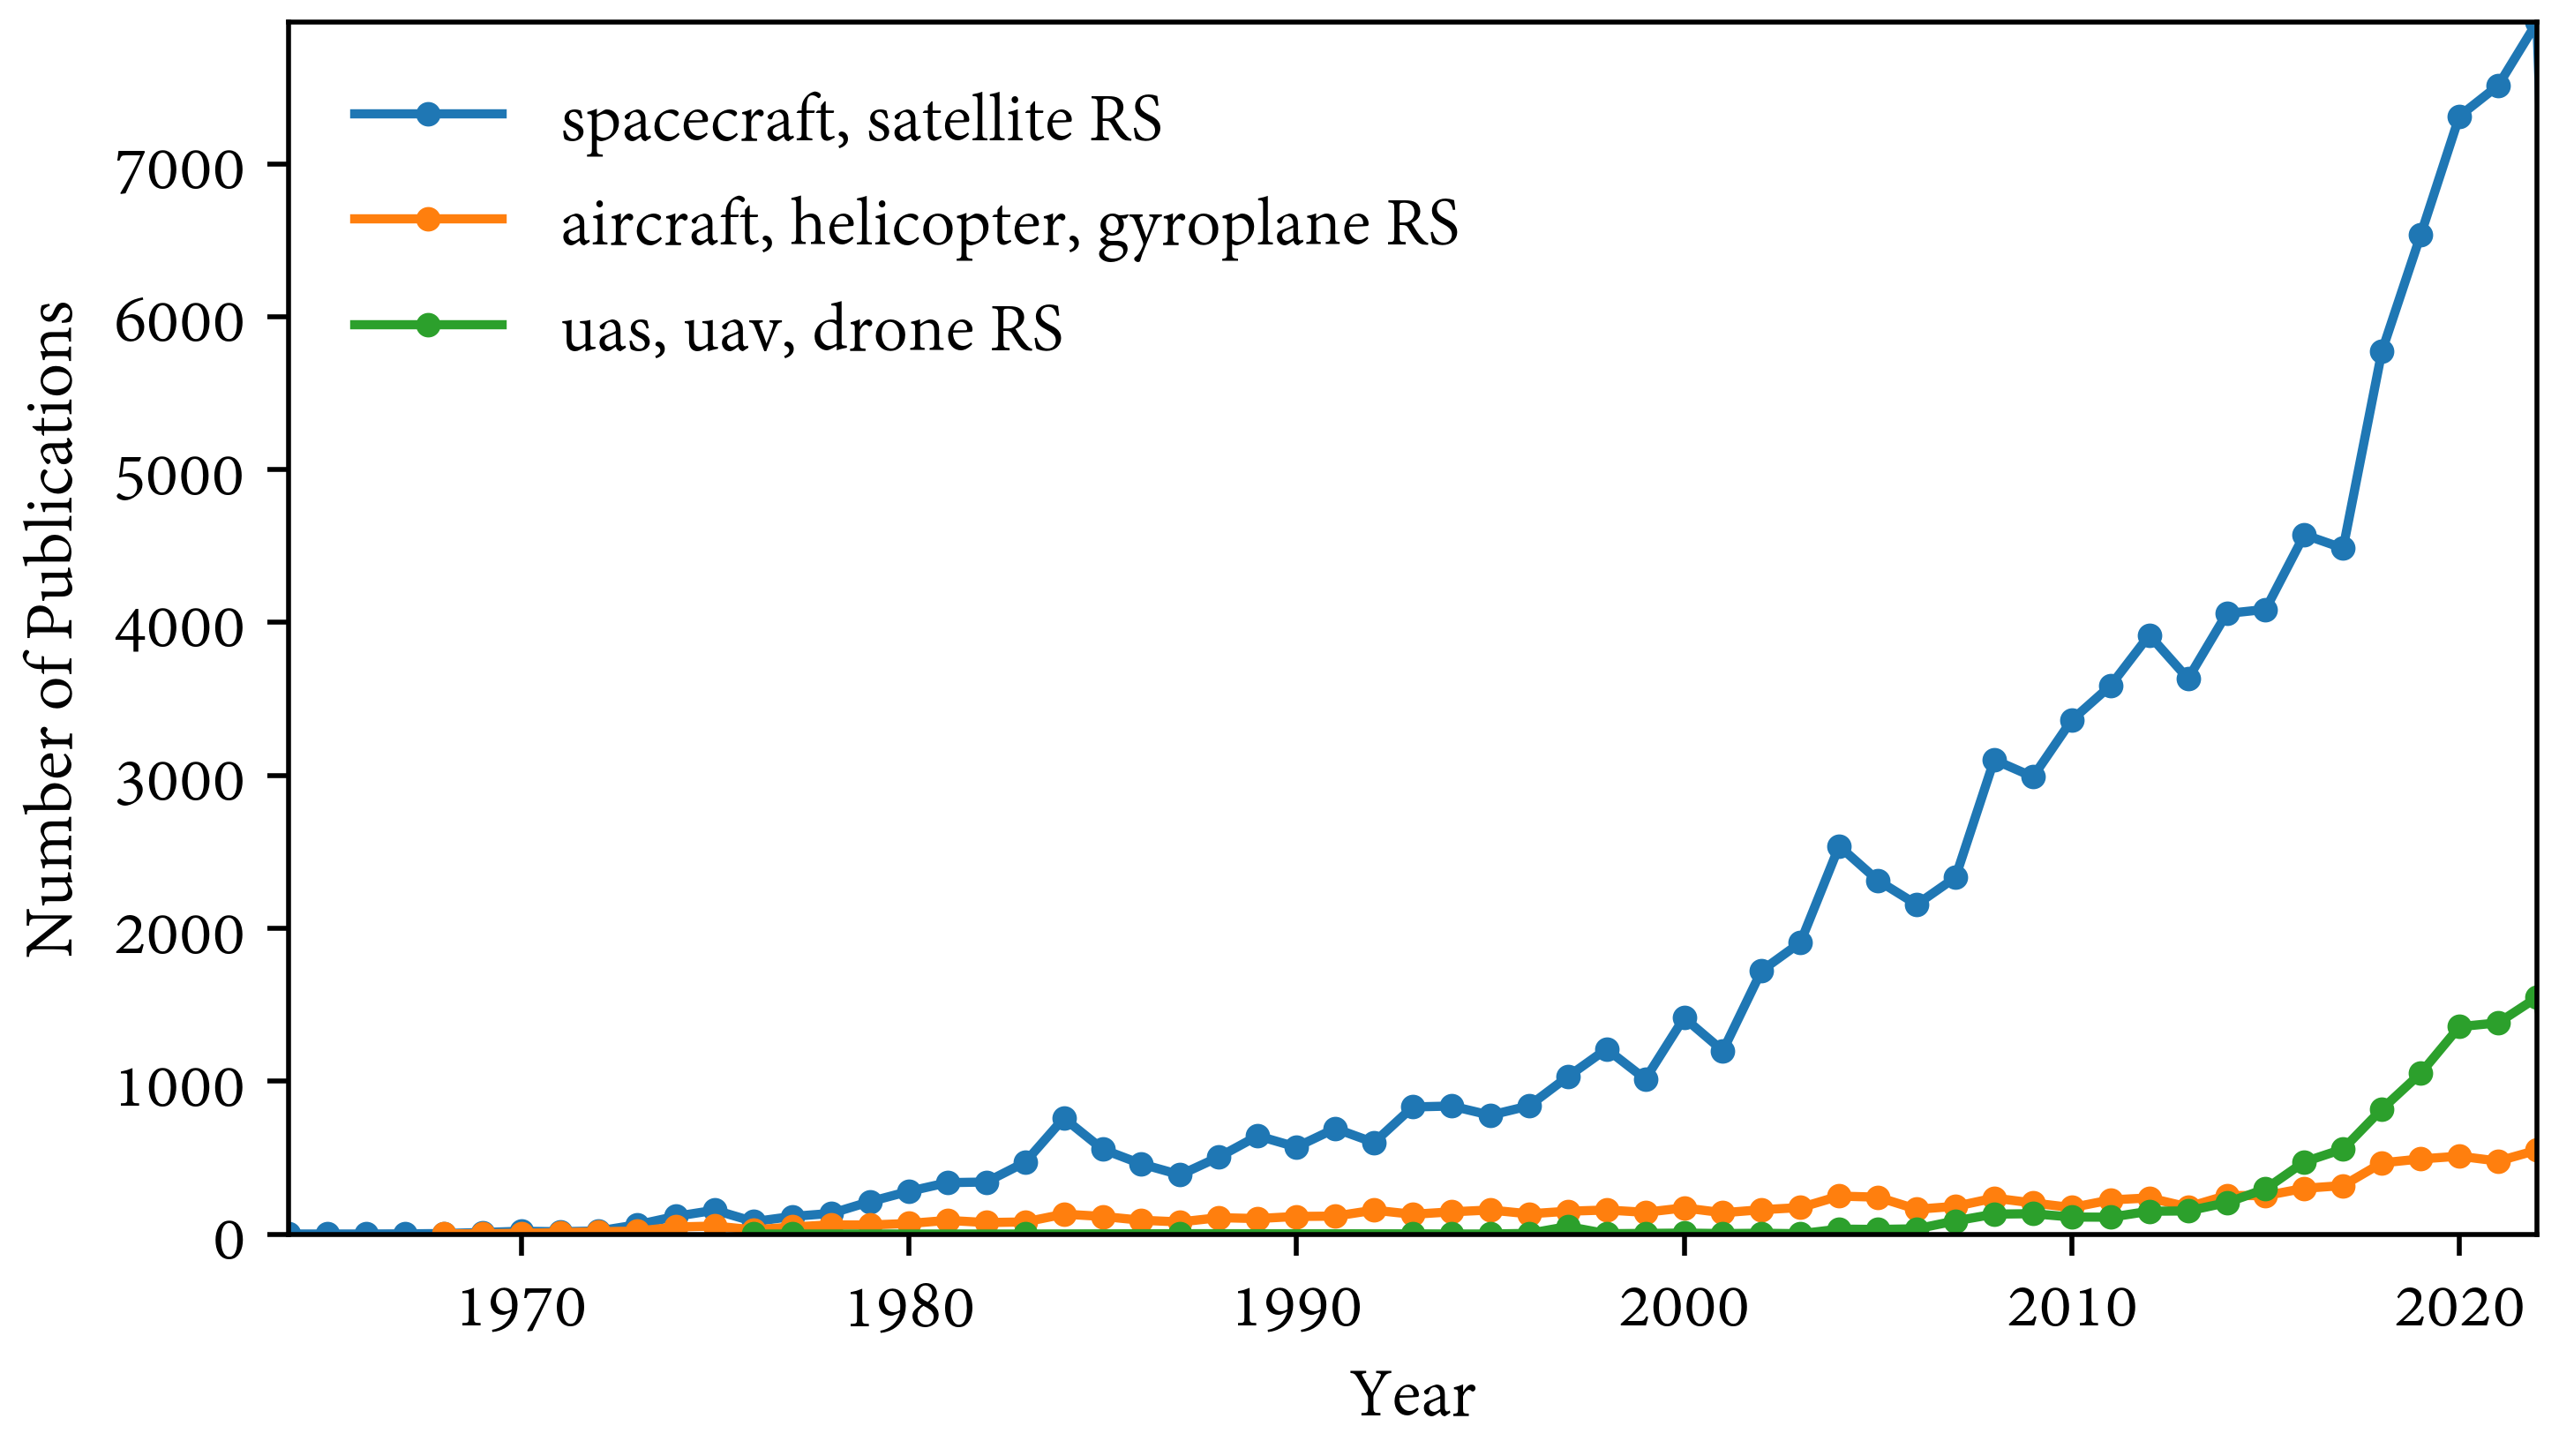
\includegraphics[width=\linewidth]{figs/introduction/platform_timeline.png}
	\caption{Número de artículos relacionados con diferentes plataformas de teledetección. Las búsquedas de Scopus fueran las siguientes: $(p_1 \lor p_2 ... \lor p_n) \land (\textit{remote} \hspace{1mm} \land \hspace{1mm} \textit{sensing})$, donde $p_i$ es una de las plataformas en la leyenda. }
    \label{fig:scopus_search_platforms_spanish}
\end{figure}

\begin{marginfigure}[.7cm]
	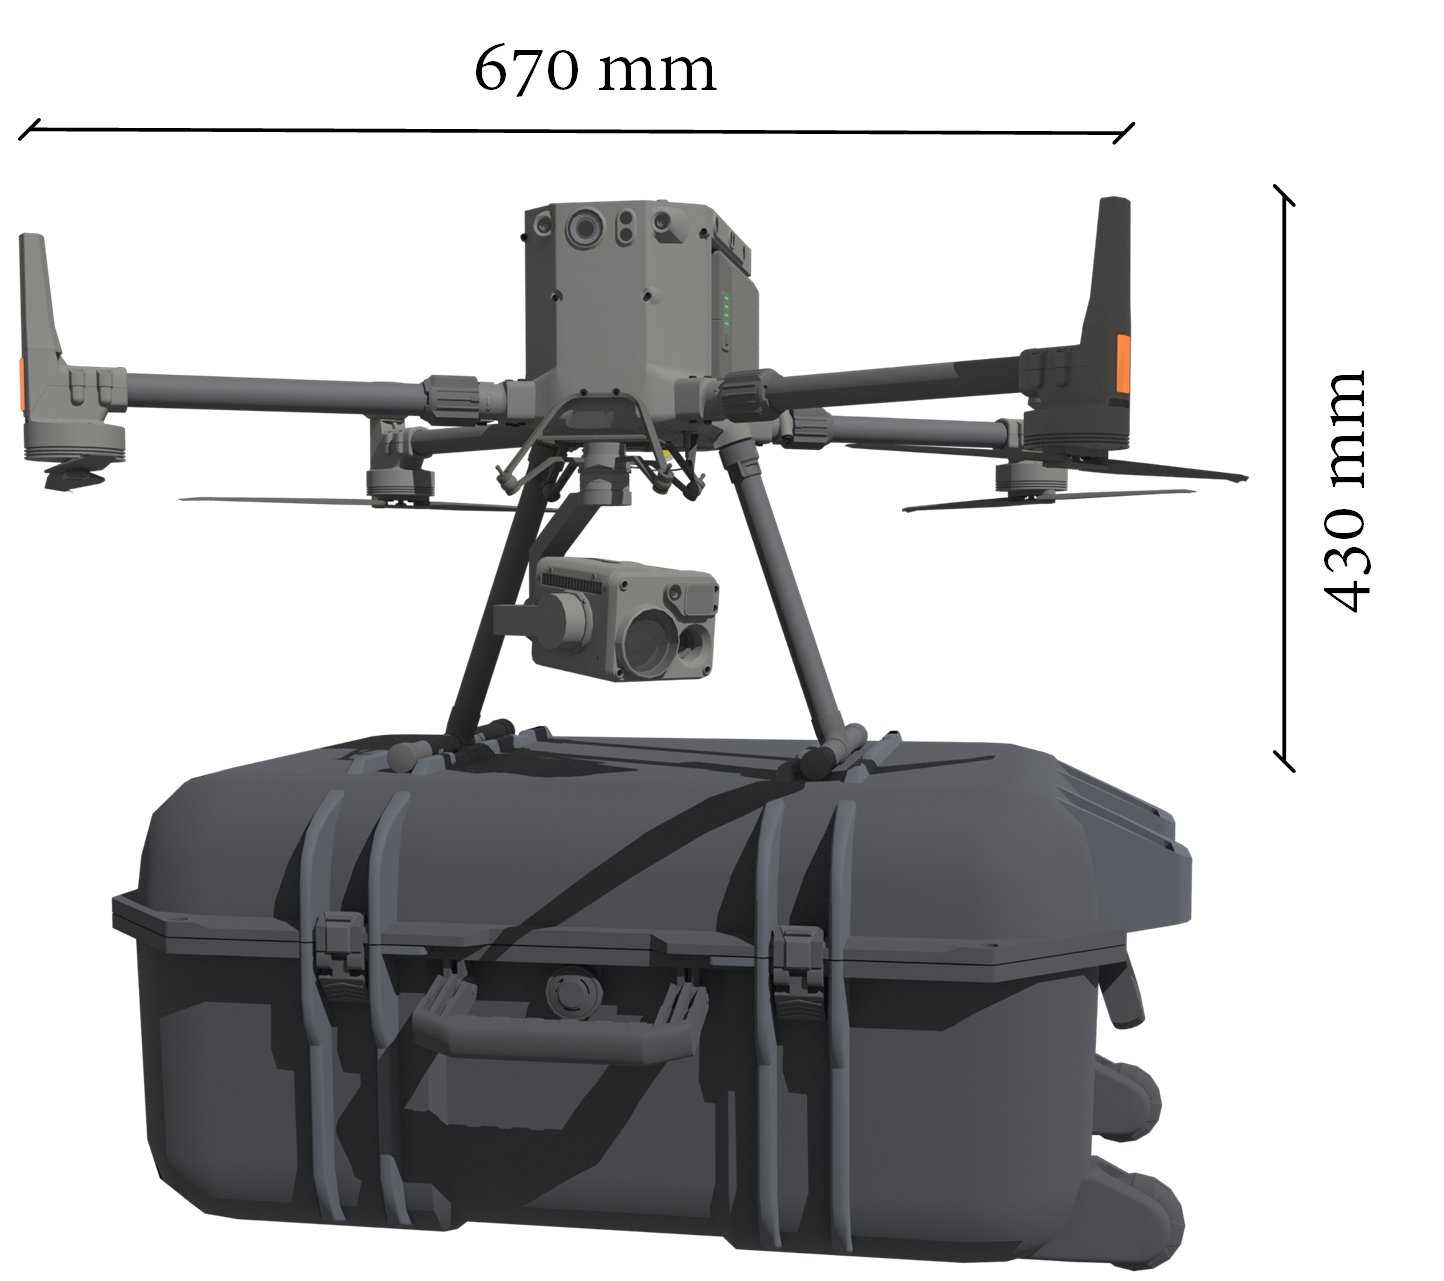
\includegraphics{figs/introduction/dji300.png}
	\caption{Quadcóptero Matrice 300 RTK, acoplado con un dispositivo dual RGB-termográfico. }
	\label{fig:dji300_spanish}
\end{marginfigure}
Además de las dificultades técnicas, la resolución de las misiones de satélite se encontraba restringida hasta hace muy poco por algunos gobiernos. Estas restricciones, así como las limitaciones descritas, condujeron al uso de plataformas alternativas. Además de satélites, las aeronaves (ala fija y helicópteros), los sistemas aéreos no tripulados (Unmanned Aerial Systems: \acrshort{uas}) (figura \ref{fig:dji300_spanish}) y otras plataformas terrestres (móviles y estáticas con detección próxima) son las más frecuentes \cite{lillesand_remote_2015}. La elección de cualquiera de ellas siempre implica balancear maniobrabilidad, cobertura terrestre, resolución espacial, precisión espacial, coste y campo de visión (\acrshort{fov}). Sin embargo, los drones han ido ganando interés en la última década al pasar de ser simples herramientas militares a principios de la década de los 2000, a sistemas fáciles de desplegar, pequeños y de bajo coste, ampliando así su campo de aplicación a la población civil y la investigación. Estas plataformas abarcan desde aeronaves del tamaño de una mano hasta otras de gran tamaño que pueden ser controladas por operadores humanos, o incluso ser parcial o totalmente autónomas. La figura \ref{fig:dji300_spanish} muestra un dron estándar diseñado por DJI que puede transportar hasta 2,7 \si{\kilo\gram}, con unas dimensiones de $501 \times 403 \times 252$ \si{\milli\meter}.

\begin{figure}[!ht]
	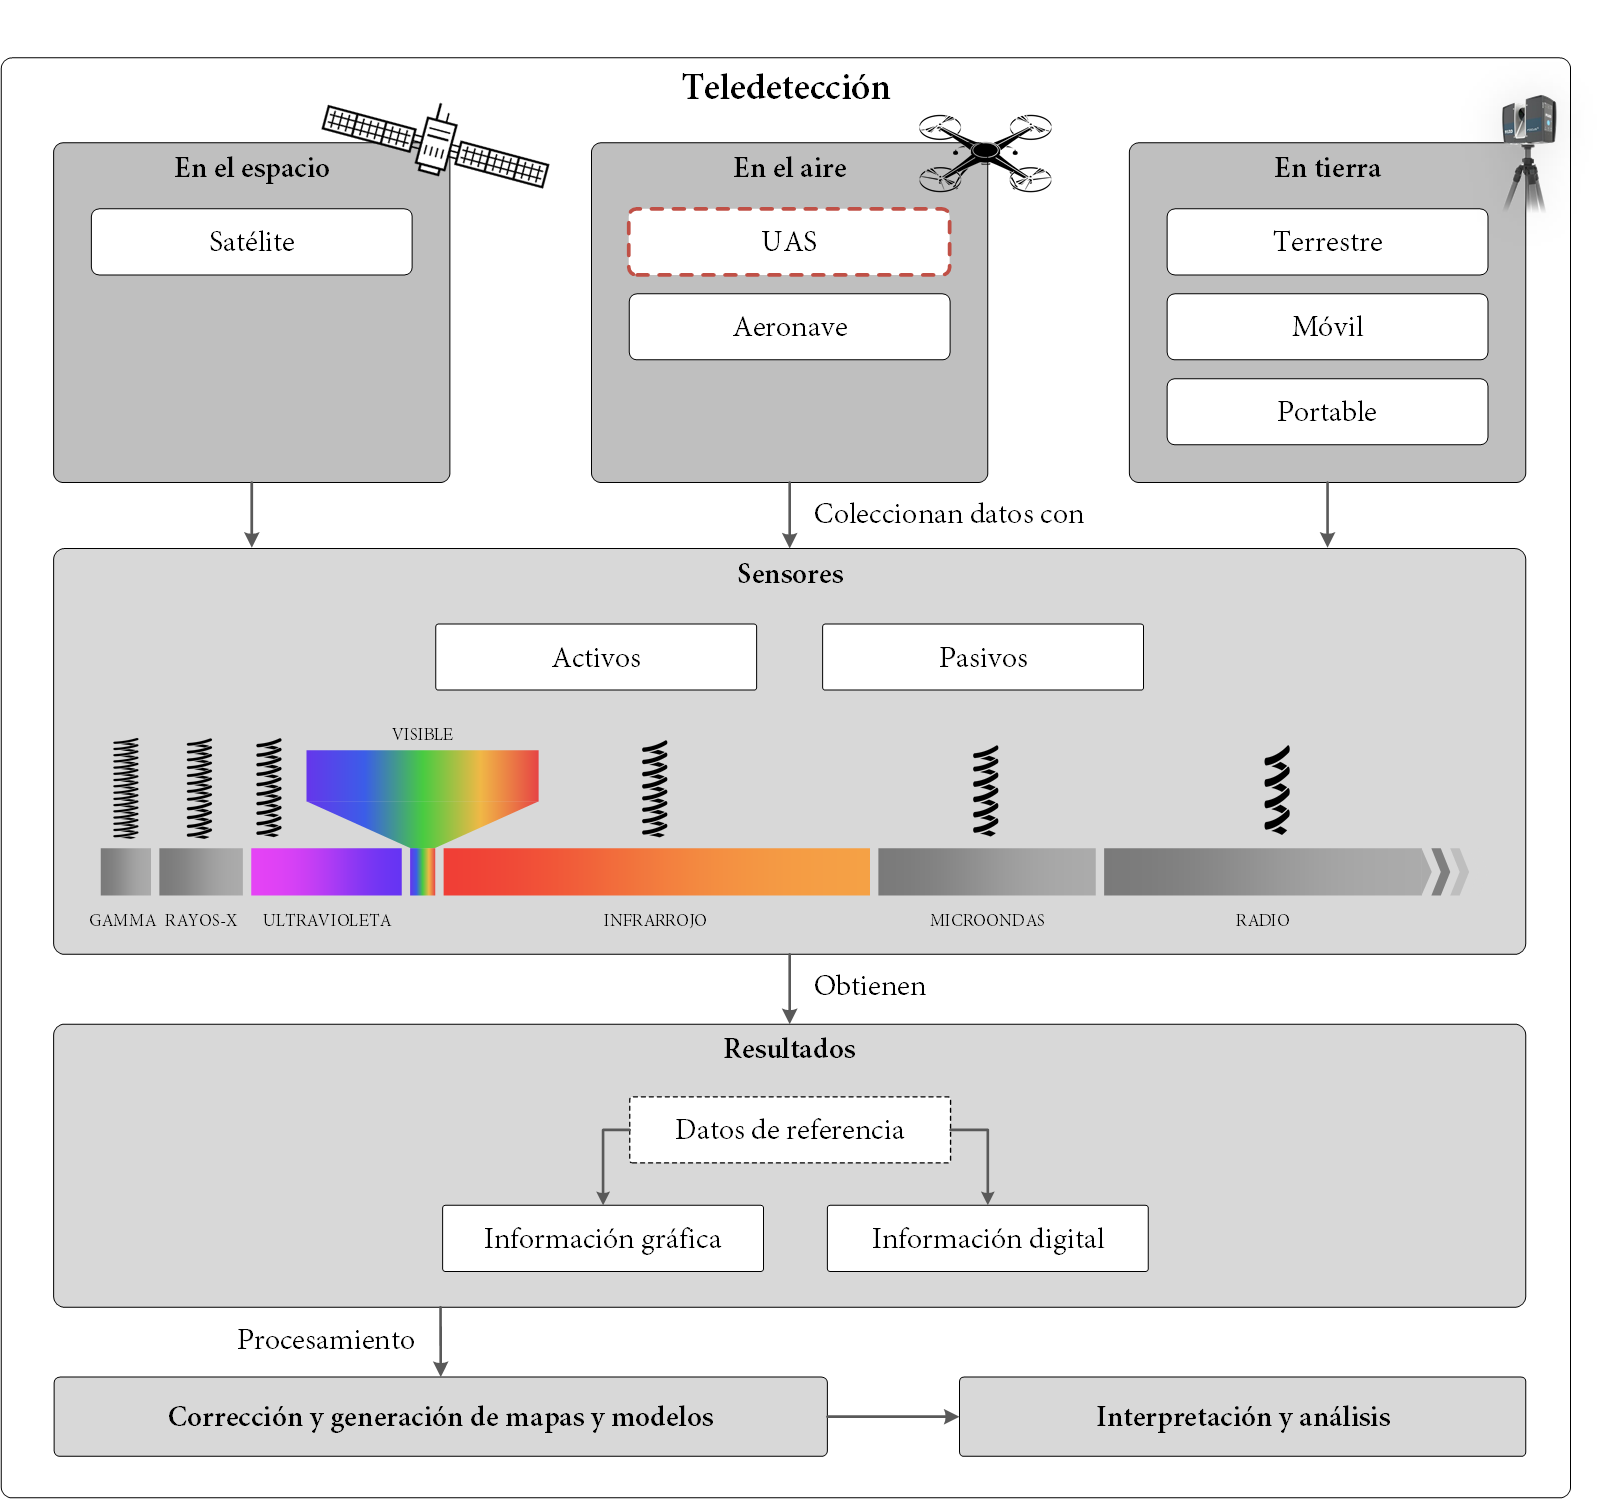
\includegraphics{figs/introduction/introduction_scheme_spanish.png}
	\caption{Procedimiento general de adquisición de datos con plataformas y sensores de teledetección. En primer lugar, los sensores se acoplan en vehículos espaciales, aéreos y terrestres, o son manejados por humanos. A continuación, los productos obtenidos pueden agruparse en resultados gráficos y numéricos, aunque la mayoría de ellos producen ambos tipos de datos. Por último, dichos productos se procesan e interpretan para proporcionar a los usuarios un análisis determinante en el control de algún proceso. }
    \label{fig:introduction_scheme_spanish}
\end{figure}

Los componentes más frecuentes de un dron destinado a la teledetección son los sensores ópticos así como los sistemas de navegación y comunicación. Estos últimos permiten al operador desplazar la plataforma dentro de un rango de comunicación, y transferir datos en un canal bidireccional. Independientemente de la ruta de navegación, ya sea manual o establecida mediante algunos puntos de control, se emplean Sistemas de Posicionamiento Global (Global Positioning System: \acrshort{gps}) y Unidades de Medición Inercial (Inertial Measurement Unit: \acrshort{imu}) para calcular y registrar la posición, orientación y movimiento de la nave. Estos componentes son especialmente relevantes para realizar misiones con un alto grado de precisión, el cual se determina mediante el error vertical y horizontal en metros (\si{\meter}). En este sentido, las últimas series de drones de DJI especifican errores verticales y horizontales por debajo del metro mediante el uso de posicionamiento cinemático en tiempo real, en lugar de \acrshort{gps}. Como es de esperar, aquellos drones que integran sistemas de navegación más ligeros y con mayor precisión son más caros.    

En términos de normativa de seguridad, el término \acrshort{uas} no sólo se refiere al propio vehículo, sino también a los sensores acoplados. Los sensores que suelen integrarse en aeronaves varían en función de la altitud de vuelo y la velocidad de crucero de la plataforma, así como de los requisitos del caso de estudio. Los vehículos de ala fija y rotatoria están mucho más limitados en altura y velocidad respecto de otras plataformas tales como helicópteros y autogiros. Aparte de las propias limitaciones de la plataforma, la altitud de vuelo puede estar limitada por normativa para evitar entrar en el dominio aéreo de otros vehículos. Por ello, los sensores y las misiones que requieren menor velocidad, menor altitud de vuelo y, por tanto, mayor precisión, son especialmente convenientes para drones. Un ejemplo muy extendido de esto mismo en teledetección es la monitorización de torres y líneas de transmisión, éstas últimas con una estructura muy fina. Por tanto, este caso de estudio requiere un proceso de toma de datos mucho más lento. En comparación, otras tecnologías, como InSAR (Interferometric Synthetic Aperture Radar), se han aplicado principalmente a misiones espaciales para rastrear cambios en la superficie terrestre.
\marginnote[-6.0cm]{La operabilidad de las aeronaves no tripuladas en la Unión Europea está regulada por el reglamento 2019/947. Entre otras restricciones, la altitud máxima de vuelo se limita en 120 \si{\meter} sobre la superficie terrestre, salvo que sobrevuele un obstáculo.} 

Por lo tanto, los drones son una herramienta de bajo coste para adquirir datos de alta resolución. Los sensores que más comúnmente se integran son las cámaras y los sensores \acrshort{lidar} (Light Detection and Ranging). Del mismo modo, esta clasificación también da lugar a la diferenciación de sensores pasivos y activos. Mientras que los sensores pasivos se basan en un sistema transmisor-receptor, los sistemas activos simplemente se limitan a captar la radiancia emitida por las superficies presentes en la escena. Sin embargo, la adquisición de múltiples fuentes de datos de alta precisión presenta ventajas e inconvenientes. 

\marginnote[6.0cm]{La digitalización de bienes, procesos y sistemas se ve considerable beneficiada de reconstrucciones que pueden realizarse a partir de datos recogidos por sensores. De esta manera, es posible conectar réplicas virtuales y físicas a través de un canal de comunicación. Esto es lo que se conoce hoy en día como gemelo digital.}
En primer lugar, las observaciones procedentes de diferentes sensores pueden interpretarse como características que permiten completar un sistema de conocimiento, donde cada una de ellas aporta información en un intervalo de longitudes de onda distinto. Además, buena parte de los algoritmos diseñados para analizar y extraer conclusiones a partir de datos de sensores se benefician de la disponibilidad de características que se complementan unas a las otras. No obstante, la contribución de todas ellas se podrá ponderar en función de cómo de importante son éstas para extraer un resultado. Salvo que se utilice un gran número de características, lo cual puede conducir inevitablemente a la llamada maldición de la dimensionalidad, se puede afirmar que es mejor tener un mayor número de características. Por otra parte, los datos de alta resolución ayudan a generar modelos más precisos que también son más fáciles de visualizar y analizar por operadores humanos. La utilización de datos con mayor densidad también implica reconstruir una geometría mucho más densa, omitiendo así menos detalles de la escena y facilitando la construcción de modelos digitales, simulando procesos y entornos reales. 

Una situación ideal en un sistema consistente de múltiples capas de información sería disponer de datos sin ruido y ubicados en un mismo sistema de referencia. Sin embargo, los sistemas de navegación presentan pequeños errores de posicionamiento que dificultan la fusión de varias capas de información. Estos errores se manifiestan en forma de diferencias relativas de traslación, rotación y escala entre datos de distintos sensores. Además, las condiciones ambientales, incluyendo composición, viento, temperatura o radiación solar, pueden variar de un vuelo a otro y por tanto, también los datos adquiridos, incluso con planes de vuelo y sensores iguales o similares. Estos cambios no sólo afectan a las observaciones realizadas durante una misión, sino también a series temporales. No obstante, estos pequeños cambios procedentes de errores de posicionamiento y orientación pueden mitigarse mediante puntos de control. Para ello, se muestrea la posición de dichos puntos con una precisión muy alta, y después, se indica dónde se encuentran representados en la imagen; por tanto, éstos deben ser fácilmente reconocibles. Otros inconvenientes son el ruido procedente de detectores defectuosos, especialmente en el caso de teledetección activa, partículas atmosféricas no deseadas o superficies cuyo comportamiento al reflejar la luz da lugar a una geometría irreal. Por lo tanto, es necesario definir un sistema capaz de fusionar con precisión múltiple fuentes de información, permitiendo su posterior procesamiento y la extracción de conclusiones fundamentadas. 

Los resultados obtenidos por sensores suelen transformarse en otros tipos de representaciones que no pueden obtenerse de una manera directa. En consecuencia, conjuntos de imágenes no son suficientes para interpretar el escenario en algunos contextos. Una visión más completa e intuitiva de un escenario se deriva de la fusión de imágenes, dando lugar a mapas 2D y puntos 3D calculados mediante la estimación de la posición y orientación de la cámara, y la búsqueda de características visibles en varias imágenes. Durante este proceso de transformación, las propiedades radiométricas y geométricas estimadas pueden sufrir una pérdida de precisión importante a consecuencia de interpolaciones de datos, por lo que este tipo de representaciones se pueden comparar con otros resultados más fiables. Por ejemplo, las nubes de puntos \acrshort{lidar} obtienen resultados tridimensionales más precisos que podrían utilizarse como medida de calidad de las nubes de puntos reconstruidas mediante imágenes. Del mismo modo, las imágenes pueden utilizarse para medir la calidad de la información radiométrica resultante.   

Por otro lado, los grandes volúmenes de datos son difíciles de manejar en términos de procesamiento, almacenamiento y visualización. Miles de imágenes o millones de puntos son difícilmente manejados en ordenadores que no se encuentran destinados a ofrecer un gran rendimiento, debido principalmente a los requisitos de almacenamiento y computación. Sin embargo, las tendencias actuales en informática han favorecido la proliferación de ordenadores personales y profesionales con gran capacidad de almacenamiento, acceso más eficiente a datos y una gran capacidad de paralelización. Esta última pueden sustentarse en la Unidad Central de Procesamiento (\acrshort{cpu}), cuya tendencia es aumentar el número de núcleos, o en la Unidad de Procesamiento Gráfico (\acrshort{gpu}), compuesta por millones de pequeñas unidades que pueden resolver tareas pequeñas de manera masiva y compartir datos entre grupos de hilos. La sección x profundiza en los formatos de datos más comunes en teledetección; en este momento, basta con imaginar estos datos como millones de números digitales (Digital Number, \acrshort{dn}). A pesar de que hoy en día el coste del almacenamiento es mucho más reducido, persisten retos tales como la recuperación eficiente y parcial de información almacenada, especialmente en aplicaciones interactivas \cite{bejar-martos_strategies_2022, ogayar-anguita_nested_2023}. 

\begin{marginfigure}[.5cm]
	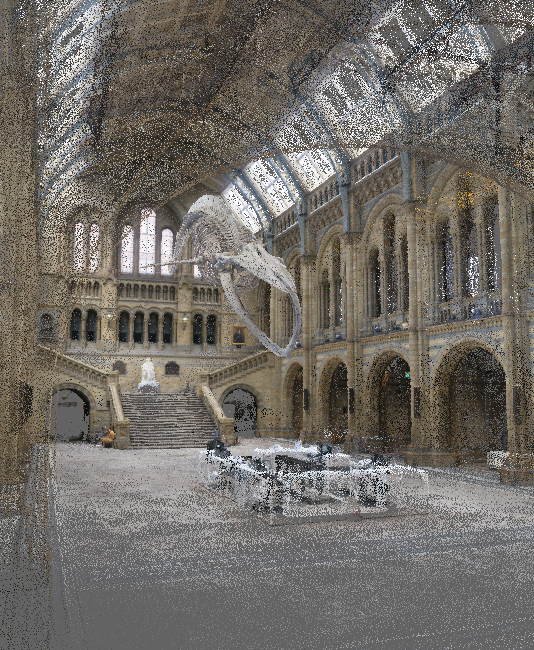
\includegraphics{figs/introduction/hintze.png}
	\caption{Nube de puntos con 2.4M de puntos reconstruidos usando 900 imágenes obtenidas de la Sala Hintze (Modelo subido por \textit{Thomas Flynn} en \textit{Sketchfab}).  }
	\label{fig:hintze_hall_spanish}
\end{marginfigure}
Otro inconveniente de las aplicaciones en tiempo real es la visualización de estos grandes volúmenes de datos. Los métodos tradicionales de rendering ejecutan conjunto de etapas inamovibles, en las que la geometría y la topología del modelo se transforman iterativamente para producir una imagen, es decir, píxeles. Los colores de éstos se calculan a partir de la influencia de una o varias fuentes de luz sobre las texturas de una superficie, discretizando así la formulación que describe la interacción de la luz. A diferencia de los modelos sintéticos diseñados por operadores humanos, los datos obtenidos por sensores se sombrean en función de la radiancia observada en un conjunto de longitudes de onda a las que es sensible el dispositivo. Por tanto, se necesitan flujos de trabajo alternativos para visualizar estos datos. De acuerdo con la arquitectura de una \acrshort{gpu}, los datos pueden ordenarse y organizarse en estructuras de datos buscando un equilibrio entre carga de trabajo y simplificaciones geométricas que ayudan a alterar la percepción del usuario. Los requisitos son aún más mayores para dispositivos de Realidad Virtual (\acrshort{vr}) que renderizan cada representación de la escena al menos una vez para cada ojo, aunque puede incrementarse en función de las técnicas de iluminación utilizadas.

\marginnote[1cm]{Esta tesis tiene como principal campo de investigación la Agricultura de Precisión y por tanto, el análisis de datos se ha acotado a 1) segmentar los cultivos en suelo y vegetación, y 2) fenotipado de un gran número de variedades vegetales de manera no destructiva.}
Los métodos anteriores no son más que un procedimiento que permiten extraer información textual o visual a partir de datos de sensores. En consecuencia, el último paso es la clasificación, segmentación e identificación de características a partir de los datos de entrada, con el fin de optimizar procesos. Las principales aportaciones de las técnicas de teledetección en la Agricultura de Precisión son la estimación del rendimiento de una plantación, la clasificación del tipo de cultivo, la medición del agua disponible, el índice de área foliar (Leaf Area Index, \acrshort{lai}) y el control de enfermedades e insectos, así como la monitorización de la humedad, cambios, crecimiento, estrés y sequía, además de otros factores de riesgo como la nieve o el fuego \cite{huang_agricultural_2018}. Con estas tareas de vigilancia se pretende maximizar la rentabilidad y minimizar los residuos y la contaminación. 

Se han publicado un número significativo de conjuntos de datos derivados de la teledetección, principalmente fomentado por el incremento de aplicaciones y algoritmos de clasificación de imágenes utilizando métodos de aprendizaje automático (Machine Learning, \acrshort{ml}) y aprendizaje profundo (Deep Learning, \acrshort{dl}) de inteligencia artificial (Artificial Intelligence, \acrshort{ai}). Por lo tanto, llevar a cabo tareas de análisis hoy en día es mucho más fácil gracias al acceso a conjuntos de datos de grandes dimensiones. Sin embargo, una gran mayoría de colecciones de imágenes obtenidas por misiones de satélite y orientadas hacia aplicaciones muy específicas, por ejemplo, a la inspección de entornos urbanos. Otro desafío es la propia clasificación de estas grandes colecciones, dado que se debe realizar mediante algoritmos no supervisados, que transforman y extraen características relevantes, o por operadores humanos \cite{li_image_2021, basu_deepsat_2015}. Ninguno de los dos métodos es perfecto y, por tanto, pueden dar lugar a datos incorrectamente clasificados que pueden inducir a error a los algoritmos de aprendizaje. Además, el etiquetado manual se suele realizar sobre bandas visibles, que son más fáciles de interpretar, y, por tanto, muy pocos conjuntos de datos incluyen bandas más allá del espectro visible. En este sentido, los sensores hiperespectrales mitigan este último problema, ya que adquieren un intervalo mucho más amplio que permite, además, obtener una imagen de falso color \acrshort{rgb}.

Aunque existen algunos conjuntos de datos disponibles para la teledetección, así como una gran variedad de sensores y bandas espectrales, éstos podrían no ser válidos para casos de estudio no tan comunes en la literatura. Para solventar esto, la solución por adquirir, de manera propia, conjuntos de datos. Sin embargo, adquirir, procesar y extraer características, incluidas etiquetas reales, conlleva mucho tiempo de trabajo debido a las tareas manuales que requieren tanto recursos informáticos como operadores humanos. Al menos de manera parcial, los datos procedentes de sensores podrían generarse sintéticamente emulando el funcionamiento del sensor. La principal ventaja es que los datos adquiridos a partir de un sensor virtual se obtienen a partir de modelos digitales en los que no existe incertidumbre. Asimismo, los modelos digitales se enriquecen con características que podrían transferirse directamente a los resultados de la detección. Los sensores simulados con más frecuencia son los sistemas Radar y \acrshort{lidar}, aunque recientemente también se han generado imágenes sintéticas con el auge de las redes generativas.

\section{Propósitos y objetivos}

De acuerdo con los retos presentados anteriormente, el objetivo general de esta disertación es contribuir en algunas de las etapas presentadas en la Figura \ref{fig:introduction_scheme_spanish}. Se han revisado brevemente un importante número de retos, entre los que se incluyen un gran número de fuentes de datos heterogéneas, las dificultades en la corrección y fusión de las mismas, la generación de productos con mayor dimensionalidad (por ejemplo, 2D $\rightarrow$ 3D) o el análisis de los resultados finales. De acuerdo con esto, los objetivos de este trabajo son los siguientes:
\begin{itemize}
    \item La corrección y el tratamiento de los datos recogidos mediante misiones de dron. Más que un único frente, este objetivo implica estudiar cómo se pueden corregir todas las fuentes de datos, incluyendo las distorsiones geométricas y radiométricas. La primera debe resolverse en la mayoría de los casos, ya que posibilita la fusión de datos, mientras que la segunda podrá ejecutarse si la radiancia se analiza posteriormente o no.
    \item El emparejamiento de imágenes recogidas por diferentes sensores, dejando atrás las diferencias relativas a 1) la distancia temporal de captura, 2) defectos ópticos, 3) el propio sistema óptico y 4) el intervalo de longitudes de onda adquirido. El emparejamiento de imágenes debe trabajar sobre imágenes con notables cambios de intensidad para obtener matrices de transformación que permitan proyectar una fuente de datos en otra. 
    \item La generación eficiente de grandes nubes de puntos 3D grandes a partir de múltiples fuentes de datos, obteniendo resultados de gran densidad y sin imprecisiones geométricas. La metodología propuesta debería abordar los inconvenientes de los métodos más notables utilizados en la fotogrametría. Además, se trata de una tarea con un alto coste computacional. Esto mismo se ve acentuado por la inclusión de múltiples fuentes de datos, por lo que debe abordarse mediante computación paralela.
    \item A pesar de que los conjuntos de datos anteriores cubren una amplia longitud de onda, éstos se amplían a 3D mediante fotogrametría para obtener un resultado más fácil de comprender. Las técnicas de fotogrametría producen resultados con menor fiabilidad que los productos obtenidos mediante sensores tales LiDAR, el cual recupera directamente la posición tridimensional de la superficie colisionada. La carencia de este sensor entre los disponibles puede resolverse emulándolo sobre escenarios 3D sintéticos. No obstante, esta tarea también requiere mucho tiempo y es especialmente difícil de modelizar en términos de intensidad devuelta. La generación eficiente de grandes conjuntos de datos LiDAR etiquetados debe abordarse, de nuevo, utilizando computación acelerada y caracterizando las superficies modeladas.
    \item La aplicabilidad de las fuentes de datos generadas previamente es el último punto de este trabajo. Entre sus aplicaciones se encuentran la detección de anomalías, la segmentación de materiales o el fenotipado de un gran número de variedades de vegetación. Puede realizarse tanto con técnicas tradicionales, como utilizando modelos de AI
\end{itemize}

\section{Organización del documento}

Esta tesis se compone de seis partes diferentes:

\small \textls[30]{PARTE I} \normalsize\hspace{3mm} Esta parte abarca este capítulo, donde se introduce al usuario la terminología empleada en la teledetección, al mismo tiempo que plantea algunos de los principales retos en este campo. Una descripción mucho más amplia de los principales sensores y procesos implicados se encuentra en el Capítulo \ref{sec:fundamentals_rs}, y posteriormente, el Capítulo \ref{sec:context_rs} ofrece una revisión del estado del arte acerca de la fusión y simulación de datos obtenidos desde dron.

\small \textls[30]{PARTE II} \normalsize\hspace{3mm} En esta parte se detallan los conceptos básicos de este trabajo, incluyendo qué tipo de sensores y datos se utilizan. Después, se describe el proceso de corrección y fusión de imágenes que será la base sobre la que se sustenta parte de este trabajo. En definitiva, esta sección engloba los materiales y métodos que comparten múltiple capítulos de esta tesis.

\small \textls[30]{PARTE III} \normalsize\hspace{3mm} Esta parte presenta la generación eficiente de nubes de puntos 3D compuestas por múltiples capas: información en el espectro visible, infrarrojo, multiespectral e hiperespectral. La información visible aporta una nube de puntos 3D de referencia, sobre la cual se proyectará el resto de información. En primer lugar, las imágenes infrarrojas se combinan con los datos del espectro visible mediante programación en la tarjeta gráfica (\acrshort{gpu}: Graphics Processing Unit). Un procedimiento muy similar se muestra consecutivamente para proyectar la información multiespectral, aunque esta última presenta algunos desafíos adicionales procedentes del registro de múltiples imágenes en intervalos espectrales muy distintos. Por último, la nube de puntos hiperespectral se genera siguiendo una metodología adaptada a unas condiciones de adquisición de datos hiperespectrales distintas de los conjuntos de imágenes previos.

\small \textls[30]{PARTE IV} \normalsize\hspace{3mm} Una vez se han fusionado los resultados de aquellos sensores disponibles, se plantea la simulación de otros sensores cuyo acceso es prohibitivo, y de los cuáles aún no disponía el grupo de investigación. Más en concreto, nos centramos en la simulación \acrshort{lidar}, utilizando escenarios sintéticos con etiquetas semánticas. La simulación \acrshort{lidar} se describe en dos capítulos, centrados en 1) la simulación de las propiedades geométricas de una nube de puntos \acrshort{lidar} (Capítulo \ref{sec:lidar_simulation}) y 2) la simulación de la radiancia observada (Capítulo \ref{sec:lidar_intensity}). Finalmente, dicha simulación se aplica la optimización de escaneos terrestres, principalmente en edificios, indicando qué posiciones son las óptimas de acuerdo a la configuración del sensor. Este proceso de optimización se describe en el Capítulo \ref{sec:lidar_optimization}, y aunque se aplica a edificios, no se plantea ninguna restricción que no permita aplicar este proceso a cualquier otro tipo de entorno.

\small \textls[30]{PARTE V} \normalsize\hspace{3mm} Esta parte muestra algunas aplicaciones de las nubes de puntos térmicas y las imágenes hiperespectrales. Las primeras se aplican a la detección de anomalías térmicas relacionadas con restos arqueológicos que pudieran haber pasado desapercibidos en prospecciones previas. Por otro lado, la información hiperespectral se corrige y procesa para ser aplicada a la identificación automática de variedades de viñedos, utilizando modelos de Inteligencia Artificial. 

\small \textls[30]{PARTE VI} \normalsize\hspace{3mm} El Capítulo \ref{sec:conclusions} concluye este trabajo mostrando los principales resultados obtenidos así como las posibles líneas futuras de trabajo.